%----------------------------------------------------------
% Main format settings
%----------------------------------------------------------
\documentclass{article}
\usepackage{graphicx}
\usepackage{authblk}
\setlength{\textwidth}{16cm}
\setlength{\oddsidemargin}{0pt}
\setlength{\evensidemargin}{0pt}
\setlength{\topmargin}{0cm}
\usepackage{caption} 
\captionsetup[table]{skip=10pt}
\usepackage{mathtools}
\usepackage{amssymb}
\usepackage{graphicx}
\usepackage{hyperref}
\usepackage[utf8]{inputenc}
 
\usepackage{listings}
\usepackage{float}
\usepackage{xcolor}
\usepackage{subfig}
\definecolor{codegreen}{rgb}{0,0.6,0}
\definecolor{codegray}{rgb}{0.5,0.5,0.5}
\definecolor{codepurple}{rgb}{0.58,0,0.82}
\definecolor{backcolour}{rgb}{0.95,0.95,0.95}
 
\lstdefinestyle{mystyle}{
    backgroundcolor=\color{backcolour},   
    commentstyle=\color{codegreen},
    keywordstyle=\color{magenta},
    numberstyle=\tiny\color{codegray},
    stringstyle=\color{codepurple},
    basicstyle=\ttfamily\footnotesize,
    breakatwhitespace=false,         
    breaklines=true,                 
    captionpos=b,                    
    keepspaces=true,                 
    numbers=left,                    
    numbersep=5pt,                  
    showspaces=false,                
    showstringspaces=false,
    showtabs=false,                  
    tabsize=2
}
\lstset{style=mystyle}
%----------------------------------------------------------
% Start of the document
%----------------------------------------------------------
\begin{document}

%----------------------------------------------------------
% Title and authors sections
%----------------------------------------------------------
\title{Dirichlet Problem: Using the Shooting Method for Solving a Boundary Value of a Region by Means of the Newton Algorithm}
\author{Bernardo A. Roque Carri\'{o}n, Jomarie Jim\'{e}nez Gonz\'{a}lez, 
    Jordan A Caraballo-Vega, Pablo Negr\'{o}n Marrero}
\affil{Department of Mathematics, UPR-Humacao}
\maketitle % this produces the title block
%----------------------------------------------------------
% Introduction
%----------------------------------------------------------
\section{Introduction}

Boundary value problems (BVP) are extremely important as they model a vast amount of phenomena and applications in science and engineering. This problem has been deeply studied in fields such as fluid mechanics to acoustic diffusion, solid mechanics to heat transfer, and computational simulations \cite{Gustafson}. A BVP consists of a system of differential equations where a set of conditions is known, and whose solutions are to be found in a specified domain. It is relevant to mention that it is opposed to the initial value problem, in which only the conditions on one extreme of the interval are known \cite{Gustafson}. BVP rise naturally in problems based on a differential equation to be solved in space, while initial value problems usually refer to problems to be solved in time \cite{Gustafson}. In fact, both ordinary and partial differential equations need boundary conditions to be solved \cite{Lutzen}. Thus, the choice of the boundary condition is fundamental for the resolution of the given system since it will determine its accuracy, and in some cases, its convergence. 

The BVP was subject of many investigations by individuals such as George Green, Karl Friedrich Gauss, Peter Gustav Lejeune Dirichlet, Carl Neumann, among others. J.C Francois Sturm and J. Liouville studied the conditions which guarantee the existence and uniqueness of BVP solutions and how boundary conditions influence them \cite{Lutzen}. The importance of the Sturm-Liouville theory falls into determining if a problem is well-posed and how it is possible to computationally obtain a solution given its conditions. Among the earliest BVP to be studied is the Dirichlet problem. This BVP problem was initially intended to find the harmonic functions, particularly solutions to the Laplace's equation. Its main purpose is to find the solution of a second-order elliptic equation which is regular in the domain \cite{Rajurkar}. The Dirichlet problem for harmonic functions always has a solution, and that solution is unique, when the boundary is sufficiently smooth and \textit{f(s)} is continuous. This implies that the existence of a solution depends on the smoothness of the boundary and the given data \cite{Yanushauskas}.

A common technique used to solve the Dirichlet problem is the shooting method. This numerical method solves the BVP by dividing it into various initial value problems. In this work, we study the Dirichlet problem for given conditions along the boundary of the domain in the x-y plane. A set of steps to find the solutions of these systems will be discussed as well. The shooting method and Newton's algorithm were implemented as the numerical methods to find the solutions of given BVPs. A set of Octave scripts were developed to computationally calculate the finite solutions for the proposed systems, together with tests to prove their accuracy given real solutions. At the end, a set of possible sources of errors are described and analyzed for the future improvement of this method.

\section{Materials and Methods}

This section describes the processes and techniques used to model and solve the Dirichlet BVP. The cases studied in this manuscript have been taken from a lecture given by professor P. Negr\'{o}n as a requirement for the Numerical Analysis class \cite{Negron}. This project prioritizes the use of numerical methods for the analysis of the Dirichlet BVP and the solution of non-linear systems.

\subsection{Software}

Scripts developed for this work were generated using Octave. The function ode45, a black-box ODE solver, was used to find numerical solutions of the proposed differential equations systems. This specific function was selected due to its ability to automatically adapt the time-step according to specified absolute and relative error tolerances. A Newton function was provided by professor P. Negr\'{o}n for finding roots from given systems. No additional packages are required to run the scripts provided by this manuscript.

\subsection{Dirichlet Boundary Value Problem Formulation}

The general Dirichlet-type BVP for a function $y(t)$ in an interval [a,b] is given by:

    \begin{equation}\label{1}
        \begin{cases}
            y''(t)=f(t,y(t),y'(t)), \ \ \ \ \ a < t < b,\\
            y(a)=\alpha, \ \ \ \ \ y(b)=\beta,
        \end{cases}
    \end{equation}

where $\alpha, \beta$ are given numbers. This two-point BVP can be solved by forming a combination of the solutions to two initial value problems. A common technique for solving this type of problem is the \textit{shooting method} (see Section 2.4 for more details). Let $y(t,\gamma)$ be the solution of the initial value problem:
    
    \begin{equation}\label{2}
        \begin{cases}
            y''(t)=f(t,y(t),y'(t)),  \ \ \ \ \ a < t < b,\\
            y(a)=\alpha,  \ \ \ \ \ y'(a)=\gamma
        \end{cases}
    \end{equation}

The main idea of the shooting method is to find a value for $\gamma$ such that $y(b,\gamma)=\beta$. Thereby, we can find a root $\gamma*$ from the equation $y(b,\gamma)-\beta=0$. Let's define the function

    \begin{equation}\label{3}
        g(\gamma) \equiv y(b,\gamma) - \beta
    \end{equation}

thus we can approximate a root $\gamma*$ of g with the Newton numerical method. Note that each evaluation of the function $g$ requires the solution of the initial value problem (\ref{2}). Also, it is necessary to find $g'(\gamma)$ in order to use Newton's method. Taking the derivative in (\ref{3}) with respect to $\gamma$, we have that $g'(\gamma) = u(b)$, where:

    \begin{equation}\label{4}
        u(t)=\frac{\partial y}{\partial \gamma}(t,\gamma)
    \end{equation}

Note that the dependency of $u$ in $\gamma$ is being omitted for simplification purposes. Then, by finding the derivative of the initial value problem (\ref{2}) with respect to $\gamma$, it can be concluded that $u(t)$ is the solution of the following initial value problem:

    \begin{equation}\label{5}
        \begin{cases}
            u''(t)=\frac{\partial f}{\partial y}(t,y(t,\gamma),y'(t,\gamma))u(t)+\frac{\partial f}{\partial z}(t,y(t,\gamma),y'(t,\gamma))u'(t), \ \ \ \ \ a < t < b, \\
            u(a)=0, \ \ \ \ \ u'(a)=1.
        \end{cases}
    \end{equation}

Given the function $y(t,\gamma)$, this is a linear problem for $u(t)$; thus the initial value problems (\ref{2}) and (\ref{5}) can be numerically solved in parallel.

\subsection{Selected Boundary Value Problems Formulation}

Consider the first problem defined by:

\begin{equation}\label{6}
    \begin{cases}
        y''(t)=\frac{1}{8}(32+2t^3-y(t)y'(t)), \ \ \ \ \  1<t<3, \\
        y(1)=17, \ \ \ \ \ y(3)=\frac{43}{3}.
    \end{cases}
\end{equation} 

Let $y(t,\gamma)$ be the solution of the initial value problem

\begin{equation}\label{7}
    \begin{cases}
      y''(t)=\frac{1}{8}(32+2t^3-y(t)y'(t)), \ \ \ \ \ 1<t<3,\\
        y(1)=17, \ \ \ \ \ y'(1)=\gamma,\\
    \end{cases}
\end{equation}

in which $u(t)=\frac{\partial y}{\partial \gamma}(t, \gamma)$ is the solution of initial value problem (\ref{5}), where $f(t,y(t),y'(t))$ is the function shown in (\ref{6}). Therefore, we proceed to find a root of the scalar equation

\begin{equation}\label{8}
g(\gamma)\equiv y(3,\gamma)-\frac{43}{3}=0.
\end{equation}

To calculate $g(\gamma)$ we transform (\ref{7}) to a first-order system given the following substitutions:

\begin{equation}\label{9}
    \begin{aligned}
        u_1(t)=y(t)\\
        u_2(t)=y'(t)\\
        u_3(t)=u(t)\\
        u_4(t)=u'(t)
    \end{aligned}
\end{equation}

Thus, we get the following first-order system:

\begin{equation}\label{10}
    \begin{cases}
        u'_1(t)=u_2(t)\\
        u'_2(t)=\frac{1}{8}(32+2t^3-u_1(t)u_2(t))\\
        u'_3(t)=u_4(t)\\
        u'_4(t)=-\frac{1}{8}u_2(t)u_3(t) -\frac{1}{8}u_1(t)u_4(t)
    \end{cases}
\end{equation}

where $u_1(1)=17$, $u_2(1)=\gamma$, $u_3(1)=0$, and $u_4(1)=1$. Once system (\ref{10}) is numerically solved, and the value of $g(\gamma)$ was found, we can use the Newton method to approximate a numerical root of $\gamma$* and solve the first BVP. Additional numerical and computational details are discussed in sections 2.4 and 2.5.

\newpage

The second BVP is given by: 

\begin{equation}\label{11}
    \begin{cases}
        y''(t)=\frac{1+(y'(t))^2}{1+y(t)}, \ \ \ \ \  0<t<5, \\
        y(0)=1, \ \ \ \ \ y(5)=10.
    \end{cases}
\end{equation} 

Let $y(t,\gamma)$ be the solution of the initial value problem

\begin{equation}\label{12}
    \begin{cases}
      y''(t)=\frac{1+(y'(t))^2}{1+y(t)}, \ \ \ \ \  0<t<5, \\
        y(0)=1, \ \ \ \ \ y'(0)=\gamma ,\\
    \end{cases}
\end{equation}

in which $u(t)=\frac{\partial y}{\partial \gamma}(t, \gamma)$ is the solution of the initial value problem shown in (\ref{5}), where $f(t,y(t),y'(t))$ is the function shown in (\ref{11}). Thus we proceed to calculate the root of the following equation:

\begin{equation}\label{13}
g(\gamma)\equiv y(0,\gamma)-10=0.
\end{equation}

In the same way as in the first problem, we do the substitutions in (\ref{9}) to transform (\ref{12}) to a first-order system. Therefore: 

\begin{equation}\label{14}
    \begin{cases}
        u'_1(t)=u_2(t)\\
        u'_2(t)=\frac{1+(u_2(t))^2}{1+u_1(t)}\\
        u'_3(t)=u_4(t)\\
        u'_4(t)=-\frac{1+(u_2(t))^2}{(1+u_1(t))^2}u_3(t)+\frac{2u_2(t)}{1+u_1(t)}u_4(t)
    \end{cases}
\end{equation}

where $u_1(0)=1$, $u_2(0)=\gamma$, $u_3(0)=0$, and $u_4(0)=1$. Once system (\ref{14}) is numerically solved, and the value of $g(\gamma)$ was found, we can use the Newton method to approximate a numerical root of $\gamma$* and solve the second BVP.

\subsection{Numerical Methods}

The shooting method was selected to find the solutions of the given BVPs. This method transforms the BVP into a combination of two initial value problems and proceeds to calculate the root of the equation given by (\ref{3}) \cite{Adam}. In the previous section, the original systems were transformed into first-order systems to find their numerical solutions, particularly to find the value of $g(\gamma)$. An ODE45 solver from Octave was used for these purposes. This solver uses a combination of order four and order five Runge-Kutta methods to find the numerical solutions of differential equations systems. 

Once the systems were solved and the solution of $g(\gamma)$ was found, the Newton method was applied to approximate a numerical root of $\gamma$*. This method was selected over the bisection and secant methods due to its superior order of convergence and computational speed. The availability of a continuous derivative of $f$ reaffirmed this selection. Newton's method supposes that the given function $f$, which in this problem is represented by $g(\gamma)$, is differentiable. Then, the tangent line to $f$ in the point $(x_0, f(x_0))$ is given by the equation

    \begin{equation}\label{15}
        y = f(x_0) + f'(x_0)(x-x_0) \\
    \end{equation}
    
which is also the first degree Taylor polynomial.
 
\newpage

Therefore, an approximation of $f$ can be found using this tangent line and defining $x_1$ as the x-intercept of the line. That is:

    \begin{equation}\label{16}
        x_1 = x_0 - \frac{f(x_0)}{f'(x_0)}, \ \ \ \ \ f'(x_0) \neq 0. \\
    \end{equation}

Thus, this process can be repeated as long as it is needed, obtaining the following recursion:

    \begin{equation}\label{17}
        \begin{cases}
            x_{n+1} = x+n - \frac{f(x_n)}{f'(x_n)} \ \ \ \ \ n \geq 0,  \\
            x_0 \ \ given, \\
        \end{cases}
    \end{equation}

which is generally described as a fixed point iteration. Newton's method convergence is covered by \textit{Theorem 1} \cite{Numerico}. \\

\noindent \textbf{Theorem 1}. Suppose that $f : \mathbb{R} \rightarrow \mathbb{R}$ is a function $C^2$ in a neighborhood of the scalar $\alpha$, where $f(\alpha) = 0, f'(\alpha) \neq 0.$ Then, if $x_0$ is selected close enough to $\alpha$, the interations from (\ref{17}) converge to $\alpha$. Furthermore,

    \begin{equation}\label{18}
        \lim_{n\to\infty} \frac{\alpha - x_{n+1}}{(\alpha - x_n)^2} = - \frac{f''(\alpha)}{2f'(\alpha)}
    \end{equation}

\noindent that is, $(x_n)$ converges to $\alpha$ with convergence order of $p = 2$. The proof of this theorem is discussed in detail on professor's P. Negr\'{o}n book \cite{Numerico}. \\

\noindent \textbf{Theorem 2}. Suppose $f \in C^{n+1}(\alpha, \beta)$ and $a \in (\alpha,\beta)$. Let $R_n (x) = f(x) - p_n(x)$ the error of approximating $f$ with $p_n$. Then:

    \begin{equation}\label{19}
        R_n(x) = \frac{1}{n!} \int_{a}^{x} f^(n+1)(\xi)(x-\xi)^n d\xi = \frac{f^(n+1)(c_x)}{(n+1)!}(x-a)^{n+1}, \ \ \ x \in (\alpha, \beta),
    \end{equation}

\noindent where $c_x$ is a number between $a$ and $x$. \\

Therefore, using the Taylor Theorem (\textit{Theorem 2}) we can write:

    \begin{equation}\label{20}
        f(\alpha) = f(x_n) + f'(x_n)(\alpha - x_n) + \frac{1}{2} f''(\xi_n)(\alpha - x_n)^2 \ ,
    \end{equation}

where $\xi_n$ is between $\alpha$ and $x_n$. Since $f'(\alpha) \neq 0$ and $f'$ is continuous, there exists a closed interval $I$ around $x=\alpha$ such that $f'(\alpha) \neq 0$ for $x \in I$. Therefore we can define the number $M$ as

    \begin{equation}\label{21}
        M = \frac{1}{2} \frac{max_{x \in I}|f''(x)|}{min_{x \in I}(f'(x))}
    \end{equation}

which is finite and exists. Note that the selection of the initial value $x_0$ is extremely important to guarantee convergence. From \textit{Theorem 1} and (\ref{21}), it can be observed that if $M|\alpha - x_0| < 1$, then the iterations of this method converge to the root. Unfortunately, this estimate is not practical since $M$, which is given by (\ref{21}), is in general hard or impossible to calculate. Thus, every estimate or known detail from the system is vital to improve the convergence possibilities of this method. Techniques such as plotting $f$ or using the bisection method to understand the region more precisely, could be used to approximate this value correctly and ensure convergence. 

Lastly, a heuristic criterion to stop the iterations of this method, supposing iterations ($x_n$) are close to the root $\alpha$, could be given by:

    \begin{equation}\label{22}
        Rel(x_n) = \frac{\alpha - x_n}{\alpha} \approx \frac{x_{n+1} - x_n}{x_n}.
    \end{equation}

Thus, if $|x_{n+1} - x_n| \leq |x_n|10^{-t}$ there are approximately $t$ significant numbers in $x_n$ as an approximation of $\alpha$. The main possible sources of errors of this work reside on the ODE solvers and the Newton method. In order to restrict the error coming from the solver, the parameters of absolute tolerance and max step size were set to $10^{-6}$ and $10^{-3}$ respectively. This to ensure that steps taken by the black-box ODE solver do not increase significantly the errors in the solutions. Similarly, the tolerance of the Newton method was set to $10^{-5}$, which controls the accuracy of the calculated root value. 

\subsection{Computational Approach}

A computational workflow was developed to numerically solve Dirichlet BVPs using Octave software. A set of three functions were written to begin solving the first problem given on section 2.3 by (\ref{6}). These functions follow (\ref{10}), where the first-order system is established and the derivatives of $f$ have been calculated.  

%systyu.m (ejemplo)
\begin{lstlisting}[language=Octave]
function w=sistyu(t,u)
  w=zeros(4,1);
  w(1)=u(2);
  w(2)=f(t,u(1),u(2));
  w(3)=u(4);
  w(4)=fy(t,u(1),u(2))*u(3) + fz(t,u(1),u(2))*u(4);
end 

function w=f(t,y,z)
  w=(32+2*t^3-y*z)/8;
end

function w=fy(t,y,z)
  w=-z/8;
end

function w=fz(t,y,z)
  w=-y/8;
end
\end{lstlisting}

Then, a script to represent the $g$ function was developed. This function returns an approximation of the $g(\gamma)$ and $g'(\gamma)$ values when given the boundaries of the interval, and the $\alpha$ and $\beta$ constants. 

%gfunc.m
\begin{lstlisting}[language=Octave]
function [g,gp]= gfunc(gam,a,b,alf,bet)
  y0=[alf,gam,0,1]';
  [t,u]=ode45(@sistyu,[a,b],y0);
  m=size(u,1);
  g=u(m,1)-bet;
  gp=u(m,3);
end
\end{lstlisting}

\newpage 

Once these functions are defined, we proceed to include the method to find the roots of equation (\ref{3}). The following script to apply the Newton method was provided by professor P. Negr\'{o}n:

%modified newton.m
\begin{lstlisting}[language=Octave]
    function [x,iter]=newton(f,x0,tol,itermax)
        if nargin<3
           tol=1.0e-4;
        end
        if nargin<4
           itermax=20;
        end
        
        x=x0;
        normx=0;
        normz=inf;
        iter=0;
        
        while (normz>tol*normx)&(iter<=itermax)
            [f0,fp0]=feval(f,x);
            z=-fp0\f0;
            normz=norm(z,2);
            normx=norm(x,2);
            x=x+z;
            iter=iter+1;
        end
\end{lstlisting}

where input values are the name of the function ($f$), the initial point ($x_0$), the tolerance ($tol$), and the maximum number of iterations allowed ($itermax$). This function can be called by:

\begin{lstlisting}[language=Octave]
    [X,ITER]=NEWTON('FUNC',x0,1.0e-6,100)    or
    X=NEWTON('FUNC',x0)
\end{lstlisting}

These are all the functions needed to solve the first BVP using the shooting method. Thus we proceed to develop a script to call each subroutine and solve the system numerically. The following script was developed for the first BVP: 

\begin{lstlisting}[language=Octave]
a=1.0;
b=3.0;
alf=17.0;
bet=43/3;

x=1:.1:3;
yexacta=x.^2+16./x;

tm=newton(@(x)gfunc(x,a,b,alf,bet),a)
y0=[alf,tm, 0,1]';
[t,u]= ode45(@sistyu, [a,b],y0);

plot(t,u(:,1),'k',x,yexacta,'k+')
xlabel('t'); ylabel('y');
legend('Solucion numerica', 'Solucion exacta');
\end{lstlisting}

Note that we have included a second plot in this script that do not use the Newton subroutine. This plot has been added to graph the exact solutions of the given system to validate the accuracy of the proposed set of scripts. This in order to detect propagation of errors early in the development stage. After validating these results, we proceed to solve the second problem from section 2.3 given by (\ref{11}). The new derivatives for this system were calculated and modified as follows:

\begin{lstlisting}[language=Octave]
function w=sistyu(t,u)
  w=zeros(4,1);
  w(1)=u(2);
  w(2)=f(t,u(1),u(2));
  w(3)=u(4);
  w(4)=fy(t,u(1),u(2))*u(3) + fz(t,u(1),u(2))*u(4);
end 

function w=f(t,y,z)
  w=(1+z^2)/(1+y);
end

function w=fy(t,y,z)
  w=-(1+z^2)/((1+y)^2);
end

function w=fz(t,y,z)
  w= (2*z)/(1+y);
end
\end{lstlisting}

Additional minor changes were made to the driver script in order to modify the initial constants:

\begin{lstlisting}[language=Octave]
a=0.0;
b=5.0;
alf=1.0;
bet=10.0;

tm=newton(@(x)gfunc(x,a,b,alf,bet),a)
y0=[alf,tm, 0,1]';
[t,u]= ode45(@sistyu, [a,b],y0);

plot(t,u(:,1))
xlabel('t'); ylabel('y')
\end{lstlisting}

Thus, the only functions that require modification are the initial system function and the constants of the driver.

\section{Results and Analysis}

This section includes results found by solving the two BVPs discussed in this manuscript. Numerical approximations of the solutions for each system were calculated using Octave software. Additional details have been included below.

\subsection{Selected Dirichlet Boundary Value Problems}

Using the formulation from section 2.3 and the scripts discussed in section 2.4 we were able to find the solutions of the two proposed BVPs. The first problem given by (\ref{6}) was solved using the BVP and its exact solutions; this in order to validate the accuracy of the method. It was found that the $gamma*$ calculated through the Newton method for the first boundary value problem was -14.000. Figure 1 shows both the solutions calculated by the Newton method, and the exact solutions given by $y(t)=t^2+\frac{16}{t}$. Note that the values of the numerical solution and the exact solution match very well. 

%insert image of the solution calculated by the shooting method in equation (5) here
\begin{figure}[h!]
    \centering
    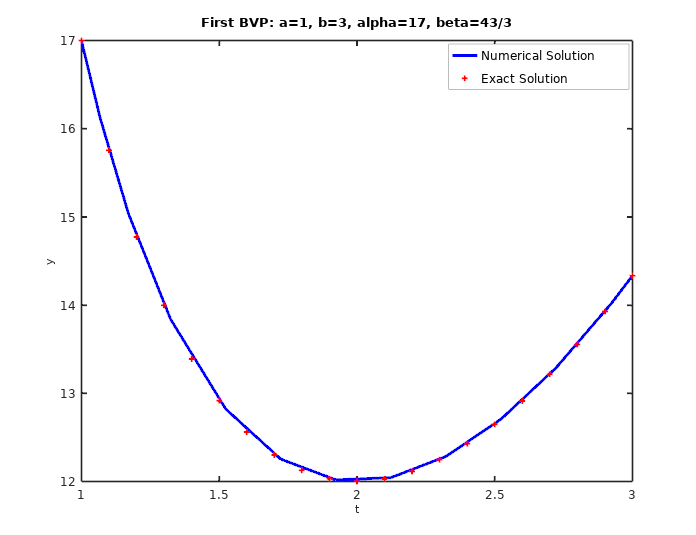
\includegraphics[width=\linewidth /2]{ejemplo1b.png}
    \caption{\textit{Exact and approximated solutions of (\ref{6}). The shooting method with initial parameters given by $a = 1.0, b = 3.0, \alpha = 17.0$, and $\beta = \frac{43}{3}$ was used for the approximation of the numerical solutions.}}
\end{figure}

\newpage

Thus we can conclude that the proposed computational approach produces accurate results and can be tested with further systems.

Same steps were followed to find the numerical solutions of (\ref{11}). The value of $\gamma*$ for this BVP was -0.12175. The exact solutions for this system were not found to validate its accuracy, but errors were kept restricted with absolute tolerance and max step size parameters. Figure 2 shows the points found x-y axis plane for this problem. In particular, compared to the first system given by (\ref{6}), this problem starts from a lower y-initial value, and it has a lower increase rate on the y-axis.

%insert image of the solution calculated by the shooting method for equation (10) here
\begin{figure}[h!]
    \centering
    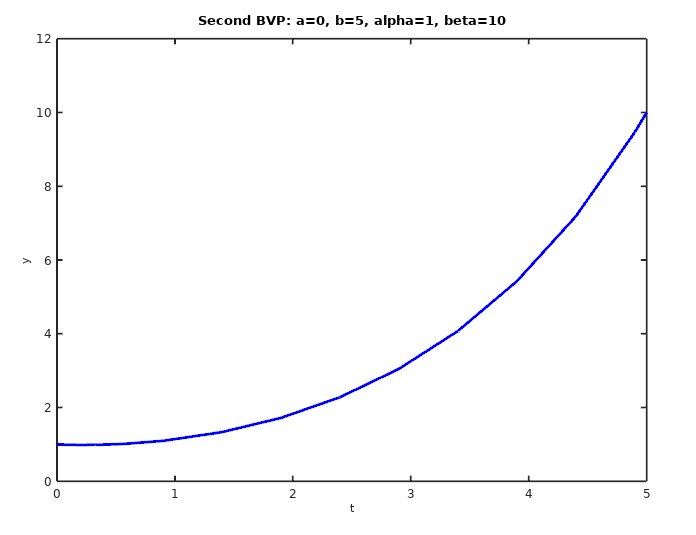
\includegraphics[width=\linewidth /2]{ejercicio3b.png}
    \caption{\textit{Approximated solutions of (\ref{11}). The shooting method with initial parameters given by \\ $a = 0.0, b = 5.0, \alpha = 1.0$, and $\beta = 10.0$ was used for the approximation of the numerical solutions.}}
\end{figure}

\section{Conclusions}

The study of the boundary value problem is of vital importance for the solution of differential equation systems. Its applicability ranges all of science and engineering fields and is present in multidisciplinary phenomena. In this manuscript we studied the Dirichlet boundary value problem by means of the shooting method. We successfully developed a computational method for calculating the approximate solutions of two boundary value problems. The Newton method was used for finding the real roots of these systems. It was discussed how this method was selected due to its superior order of convergence and speed. It was proven that the proposed method could accurately find solutions for given systems when compared to exact solutions. Errors were analyzed and restricted using absolute tolerance parameters. In conclusion, the selected numerical methods were effective to accurately calculate the solutions of two given boundary value problems. Further modifications should be done to the proposed methods to enhance its portability and version control.

\section{Future Work}

Future work includes the automation of the proposed set of scripts in order to calculate the derivatives using Matlab's symbolic libraries. Further analysis of the Dirichlet problem using additional numerical methods such as the bisection and the secant algorithms should be done to compare their accuracy against the Newton method. Finally, Neumann and Robin problems should be addressed and studied to compare the viability of these numerical methods for the calculation of accurate solutions to solve these problems.

\section{Appendices}

This section includes a set of additional resources useful for the development of this work.

\subsection{Visualizing the Boundary Value Problem}

A video including the first BVP problem discussed in this manuscript was generated and uploaded to YouTube (link=\href{https://youtu.be/nzhvtjO8vtk}{Dirichlet BVP}). Note that parameters are specified in the video description.

\subsection{Note to the Reader}

The following subsection was done to guide the reader on where to find the answers to professor P. Negr\'{o}n Boundary Value Problem lecture. 

Question 1: Answered in section 2.5. Results discussed in section 3.1. 

Question 2: Answered in section 2.5. Results discussed in section 3.1. 

Question 3: Answered in section 2.2 and 2.5. Results discussed in section 3.1. 

\begin{thebibliography}{99}

\bibitem{Gustafson}{Gustafson, Karl. \textit{Domain decomposition, operator trigonometry, Robin condition.} Contemporary Mathematics 218 (1998): 432-437.}

\bibitem{Negron}{P. Negr\'{o}n, \textit{Proyecto Computacional Final: Problema de Frontera}, UPR-Humacao, 2019.}

\bibitem{Lutzen}{L\"{u}tzen, Jesper. \textit{Sturm and Liouville's work on ordinary linear differential equations. The emergence of Sturm-Liouville theory.} Archive for history of exact sciences 29.4 (1984): 309-376.}

\bibitem{Rajurkar}{Rajurkar, R. K. \textit{General Solution of the Heat Equation, Wave Equation by Separation of Variables.}}

\bibitem{Yanushauskas}{A. Yanushauskas (2001) [1994], \textit{Dirichlet problem}, in Hazewinkel, Michiel (ed.), Encyclopedia of Mathematics, Springer Science+Business Media B.V. / Kluwer Academic Publishers, ISBN 978-1-55608-010-4}

\bibitem{Adam}{Adam, Badradeen, and Mohsin HA Hashim. \textit{Shooting method in solving Boundary Value Problem.} International Journal of Research and Reviews in Applied Sciences 21.1 (2014): 8.}

\bibitem{Numerico}{P. Negr\'{o}n, \textit{Fundamentos del An\'{a}lisis Computacional.} University of Puerto Rico at Humacao (2015)}

\end{thebibliography}


\end{document}
